\chapter{Resultados}

A continuación se presentan los resultados del sistema estudiado en esta tesis. Como se mencionó previamente, el nanotubo de carbono y moléculas de herbicida 2,4-D en presencia de agua se estudiaron a 1 bar de presión y temperatura desde 280 hasta 370 K.

% \subsubsection{Propiedades termodinámicas}

% Se muestran algunas figuras que son cálculos instantáneos de la presión y temperatura:

% \begin{figure}[!h]
%     \centering
%     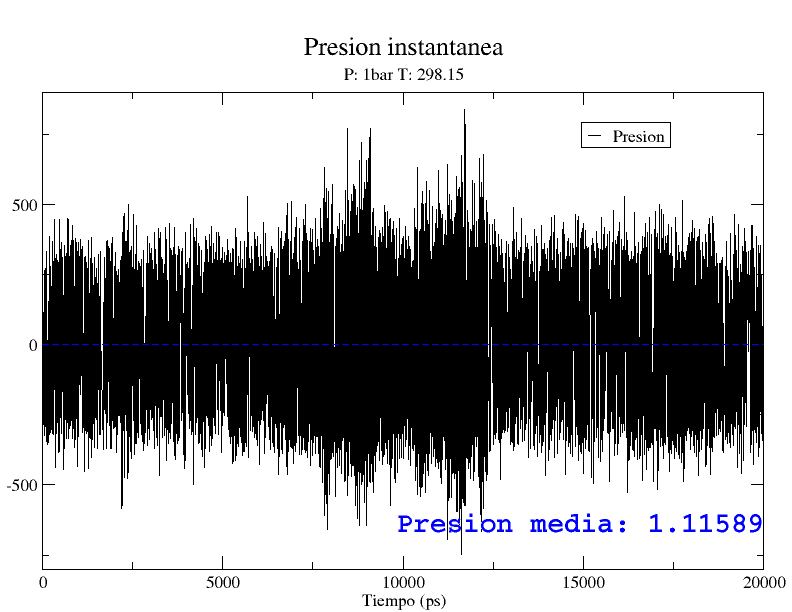
\includegraphics[width=.9\textwidth,keepaspectratio=true]{Pres298.png}
%     \caption{Gráfica de la presión instantánea del sistema a condición estandar IUPAC, la media de la presión fue 1.11589 bar}
%     \label{fig:Enertot298.15}
% \end{figure}
\section{Representación visual de la adsorción de las moléculas 2,4-D}

La figura \ref{fig:Conffinal370} es una representación visual de la adsorción de las moléculas 2,4-D en el nanotubo. Esta adsorción que se observa en la representación visual, se replica en las configuraciones finales del sistema para todas las temperaturas simuladas.

\begin{figure}[!h]
    \centering
    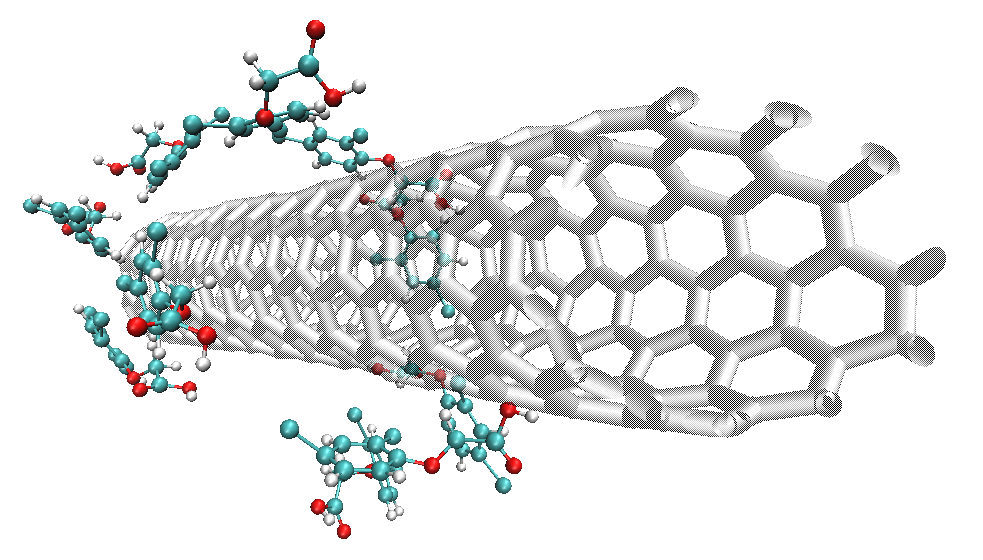
\includegraphics[width=0.6\textwidth,keepaspectratio=true]{resultados/all-new-370K.png}
    \caption{Nanotubo y moléculas de 2,4-D en la configuración final a 370 K y a 1 bar de presión.}
    \label{fig:Conffinal370}
\end{figure}

 La característica general observada en las simulaciones, es que independientemente de la configuración inicial y a medida que transcurre el tiempo, las moléculas de herbicida son atraídas hacia el nanotubo pero no ingresan dentro, lo que indica que la formación de un complejo y sugiere que el herbicida podría ser arrastrado por los nanotubos.

\section{Función de distribución radial}

Las funciones de distribución radial fueron calculadas en un rango de 280 a 370 K a 1 bar de presión. En el caso de pares átomo-átomo se calcularon los pares oxígeno-oxígeno, oxígeno-hidrógeno e hidrógeno-hidrógeno del agua, también los pares carbono del nanotubo y átomos del ácido 2,4-diclorofenoxiacético, que son carbono-oxígeno de 2,4-D, carbono-hidrógeno de 2,4-D, carbono-cloro de 2,4-D y carbono-carbono de 2,4-D. Igualmente se calcularon los pares entre el centro de masa del nanotubo y átomos de la molécula 2,4-D los cuales son centro de masa del nanotubo-oxígeno, centro de masa del nanotubo-hidrógeno, centro de masa del nanotubo-cloro y centro de masa del nanotubo-carbono. Además se calcularon la funciones para los pares centro de masa del nanotubo de carbono-centro de masa de la molécula 2,4-D y carbono del nanotubo-centro de masa de 2,4-D.\\

\begin{figure}[!h]
    \centering
    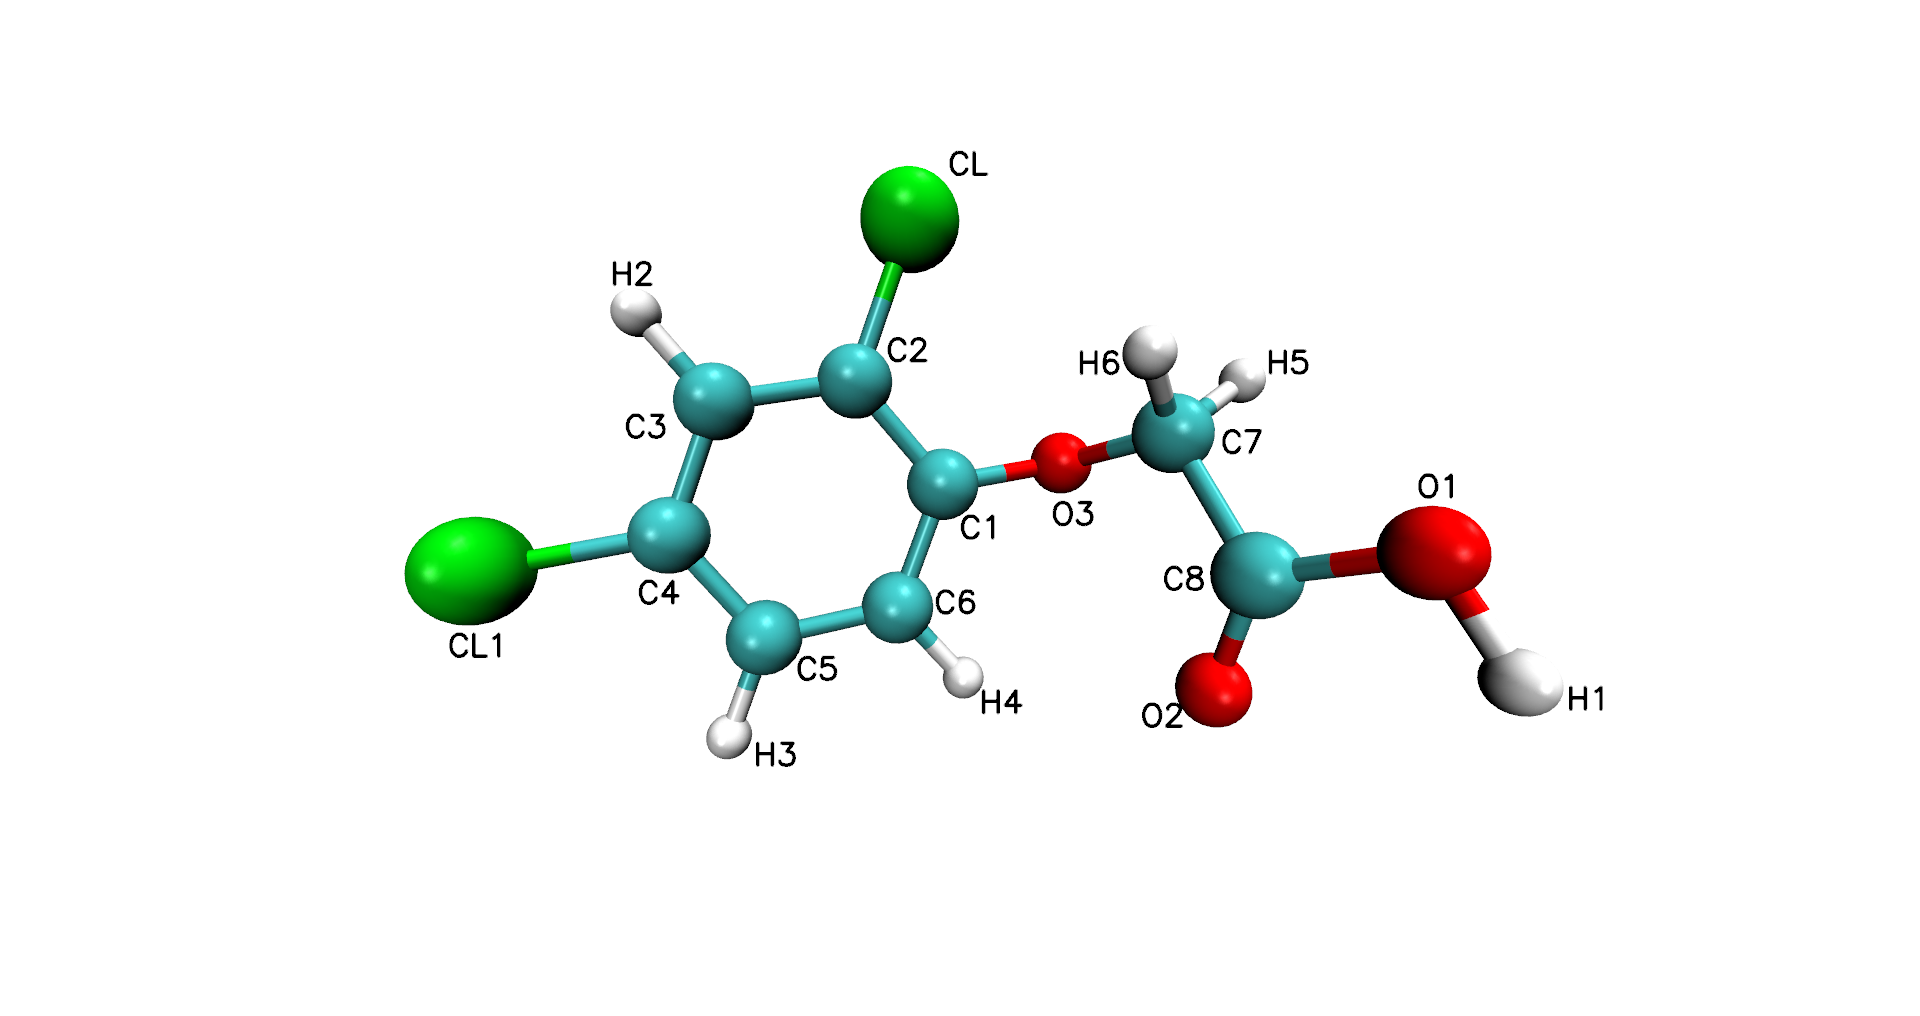
\includegraphics[width=.9\textwidth,keepaspectratio=true]{figura_nueva_tarea.png}
    \caption{Molécula 2,4-D}
    \label{fig:24Dfigureresultados}
\end{figure}

\newpage

\begin{table}[h!]
    \centering
    \begin{tabular}{ |c|l|  }
    \hline
    Tipo & Pares \\
    \hline
    \multirow{2}{*}{átomo A - átomo B} 
    & \textbf{agua - agua}: OW-OW, OW-HW, HW-HW \\ 
    & \textbf{2,4-D - CNT(6,5)}: OD-C, HD-C, ClD-C, CD-C \\ 
    \hline
    \multirow{2}{*}{centro de masa A - centro de masa B} 
     & \textbf{2,4-D - CNT(6,5)}: CNT(6,5) - 2,4-D,\\
     & tapas de CNT - 2,4-D \\
    \hline
    \multirow{5}{*}{centro de masa A - átomo B} 
    & \textbf{CNT(6,5) - 2,4-D}: \\
    & centro de masa CNT(6,5) - ClD, \\ 
    & centro de masa CNT(6,5) - HD, \\
    & centro de masa CNT(6,5) - OD, \\
     & centro de masa CNT(6,5) - Cl1D \\
    \hline
    \end{tabular}
    \caption{Funciones de distribución radial calculadas.}
    \label{tab:funcrad}
\end{table}
% \begin{itemize}
%     \item átomo A - átomo B:
%         \begin{itemize}
%             \item agua-agua: OW-OW, OW-HW, HW-HW
%         \end{itemize}
%         % \begin{itemize}
%         %     \item agua-2,4-D: OW-OD, OW-ClD, OW-HD, HW-HD, HW-ClD
%         % \end{itemize}
%         % \begin{itemize}
%         %     \item agua-CNT(6,5): OW-C,  HW-C
%         % \end{itemize}
%         \begin{itemize}
%             \item 2,4-D-CNT(6,5): OD-C, HD-C, ClD-C, CD-C
%         \end{itemize}
%         % \begin{itemize}
%         %     \item 2,4-D-2,4-D: OD-OD, HD-HD, ClD-ClD, CD-CD, ClD-HD, OD-HD
%         % \end{itemize}
%         % \begin{itemize}
%         %     \item CNT(6,5)-CNT(6,5): C-C
%         % \end{itemize}
%     \item centro de masa A - centro de masa B:
%         \begin{itemize}
%             \item 2,4-D-CNT(6,5): centro de masa CNT - centro de masa 2,4-D, centro de masa de ambas tapas CNT - centro de masa 2,4-D
%         \end{itemize}
%     \item centro de masa A - átomo B:
%         \begin{itemize}
%             \item CNT(6,5)-2,4-D: centro de masa CNT - ClD, centro de masa CNT - HD, centro de masa CNT - OD, centro de masa CNT - Cl1D
%         \end{itemize}
%         % \begin{itemize}
%         %     \item agua-2,4-D: OW-OD, OW-ClD, OW-HD, HW-HD, HW-ClD
%         % \end{itemize}
% \end{itemize}

% A continuación se presentan algunas gráficas y figuras significativas para posteriormente para analizar.\\

% \newpage

\begin{figure}[!hbt]
    \centering
    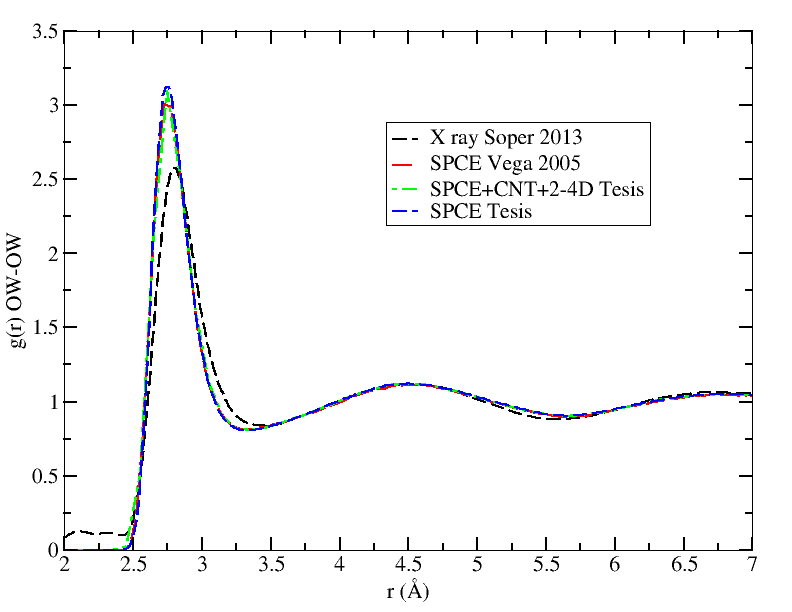
\includegraphics[width=0.7\textwidth,keepaspectratio=true]{resultados/gOOcartel.png}
    \caption{Función de distribución radial O-O de agua a 1 bar de presión: comparación entre resultados experimentales de \cite{Soper2013}, simulación de agua SPCE a 300 K \cite{vega2005}, nuestra simulación de agua SPCE a 298.15 K, y función calculada de la mezcla de la tesis a 298.15 K.}
    \label{fig:OO}
\end{figure}

\newpage

En la figura \ref{fig:OO} se presenta una comparación de la función distribución radial del par oxigeno-oxigeno de agua: la línea negra corresponde a la función experimental obtenida por Soper \cite{Soper2013} a 298 K, las líneas de color roja y azul corresponden a funciones obtenidas en simulación de agua pura de Vega \cite{vega2005} a 300 K y de nosotros a 298.15 K, respectivamente; la línea verde corresponde a la función obtenida en la mezcla simulada en este trabajo.\\

Observamos un acuerdo entre funciones de distribución radial obtenidas a través de simulación. Las diferencias observadas entre la función del modelo SPCE y la función experimentalmente alrededor del primer máximo han sido señaladas por otros autores y se confirman en nuestro estudio. Sin embargo hay un buen acuerdo a distancias mayores a 3.5 \AA. Esta característica del modelo SPCE ha propiciado su utilización en diversos estudios de simulación molecular y es uno de los más usados. Por lo tanto, el agua mantiene su estructura ya sea en simulaciones de agua pura en la mezcla nanotubo/herbicida/agua, indicando que a esta concentración de herbicida y nanotubo, la estructura de agua no se modifica sustancialmente.\\
% En la figura \ref{fig:24D_CNT_298_15_atom_atom} comparamos diferentes funciones de distribución radial a 298.25 K que se caracterizan como: carbono del nanotubo - átomo de 2,4-D. La función Cl(2,4-D)-C(CNT) y C(2,4-D)-C(CNT) tienen una distribución similar con dos máximos en aproximadamente $4.3<r1<4.5$ y $10.8<r2<11$ angstroms(\AA); y los pares  H(2,4-D)-C(CNT) y O(2,4-D)-C(CNT) tienen similares máximos con dos máximos en $r=5$ y $r=10.62$ \AA. Además, se puede observar que el hidrógeno de 2,4-D se encuentra mas cercano al carbón del nanotubo en $r\sim 2.3$\AA y el mas probable de los átomos en ser encontrado es el carbono de 2,4-D dado otro carbono en $r\sim 4.5$. \\

\begin{figure}[!hbt]
    \centering
    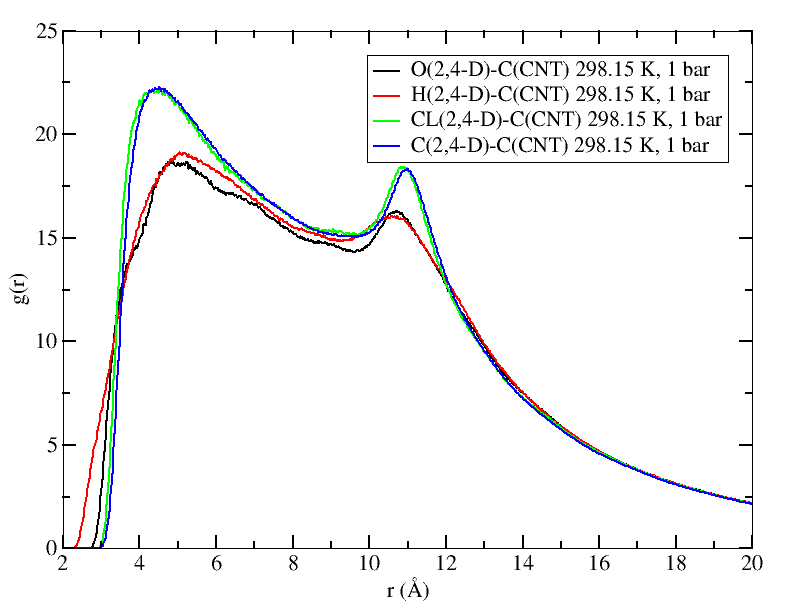
\includegraphics[width=0.6\textwidth,keepaspectratio=true]{resultados/gr_24D_CNT_298_15_atom_atom.png}
    \caption{Funciones de distribución radial átomo-átomo entre el C del nanotubo y los átomos O, H, Cl y C del 2,4-D a 298.15 K y 1 bar.}
    \label{fig:24D_CNT_298_15_atom_atom}
\end{figure}

\newpage

En la figura \ref{fig:24D_CNT_298_15_atom_atom} se compararon diferentes funciones de distribución radial a 298.25 K y 1 bar del tipo átomo-átomo. Las curvas azul y verde corresponden a las funciones carbono del nanotubo-carbono de 2,4-D y carbono del nanotubo-cloro de 2,4-D, respectivamente. \\

Observamos que son similares con dos máximos en la distribución localizados aproximadamente en 4.3 y 11 \AA. La curva roja corresponde al par carbono del nanotubo-hidrógeno de 2,4-D, esta función comienza a ser diferente de cero aproximadamente en 2 \AA\  y el primer máximo se encuentra en $\sim 5$ \AA; la curva negra corresponde a la función carbono del nanotubo-oxígeno de 2,4-D con un máximo alrededor de 5 \AA. Observamos que la mayor concentración de moléculas alrededor del nanotubo está entre 4.3 \AA\  y 5 \AA, y el hidrógeno de 2,4-D es el más cercano al nanotubo como las gráficas lo indican.\\

Estas observaciones nos permiten proponer que la conformación preferencial del 2,4-D con respecto al nanotubo ocurre como se presenta en la figura \ref{fig:figura-resultados-rdf}.\\

\begin{figure}[!hbt]
    \centering
    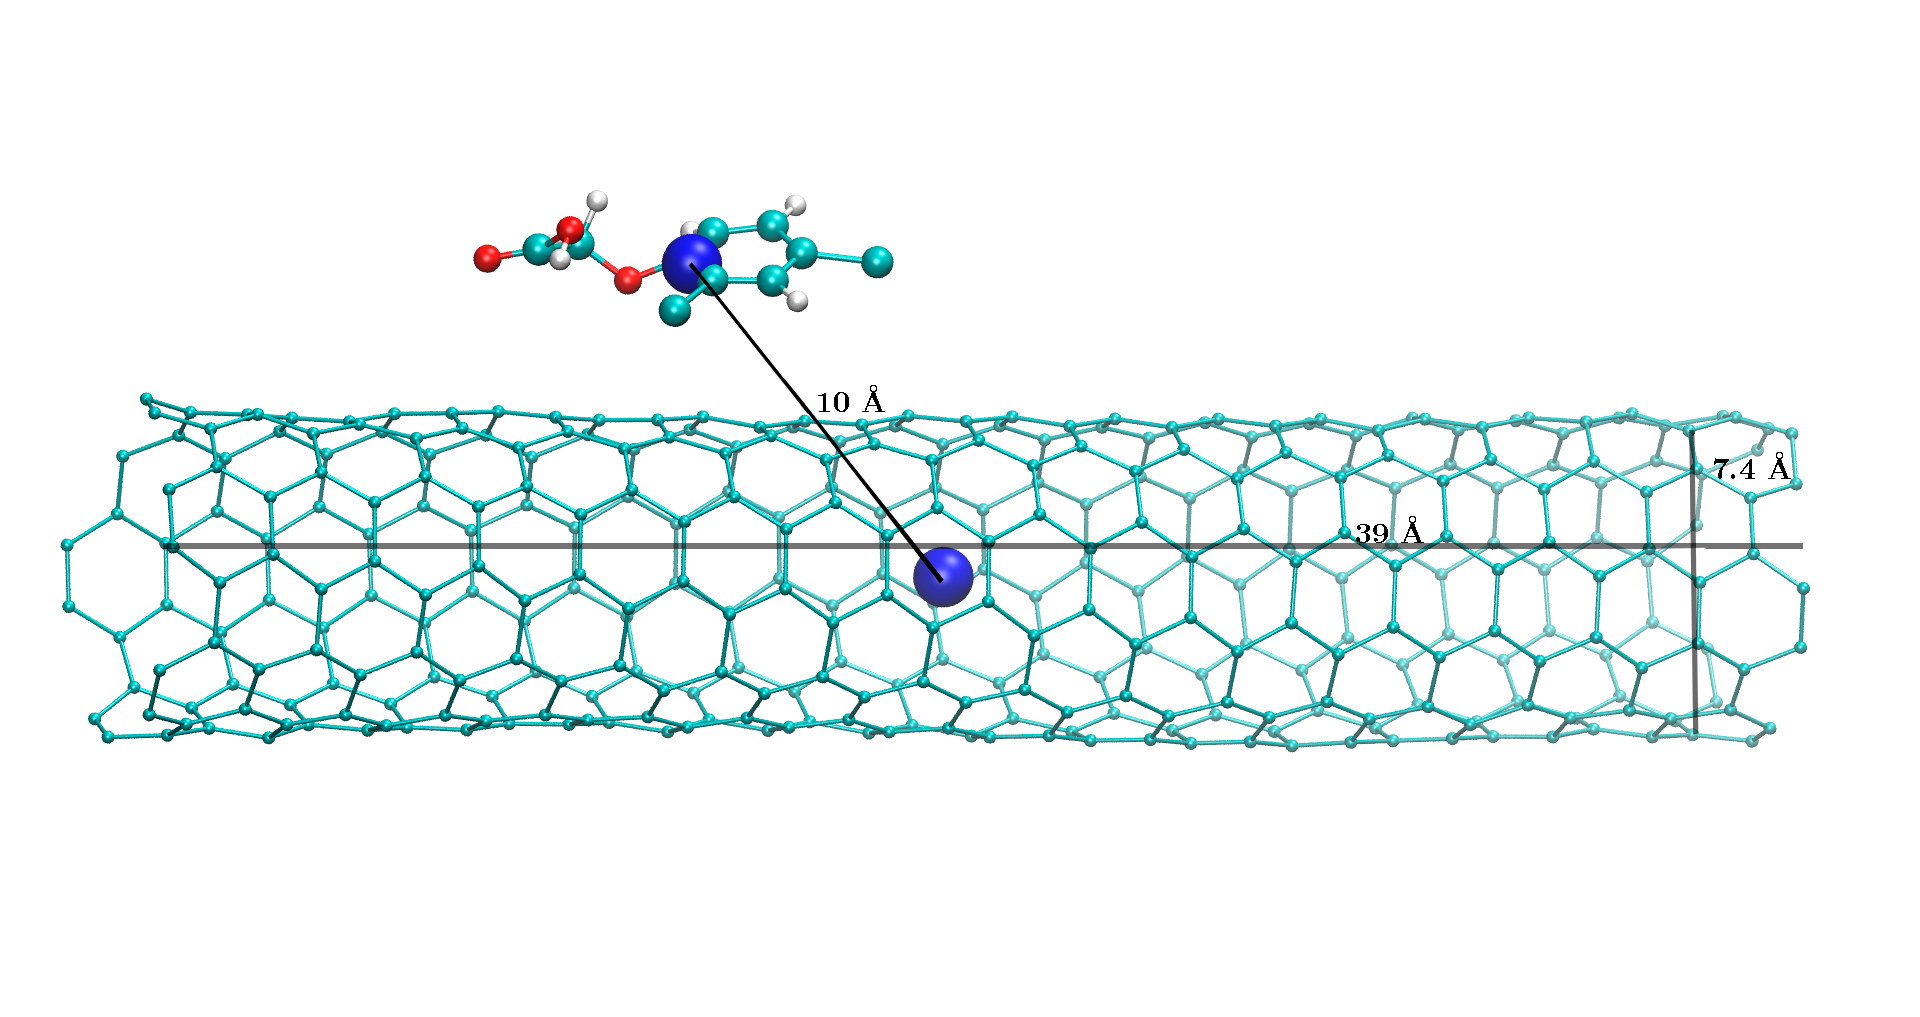
\includegraphics[width=0.9\textwidth,keepaspectratio=true]{resultados/figura-resultados-rdf.png}
    \caption{Conformación del 2,4-D con respecto al nanotubo sugerida en base a las funciones de distribución radial obtenidas con medidas estimadas de longitud, diámetro y distancia entre centros de masa del nanotubo y una molécula de 2,4-D.}
    \label{fig:figura-resultados-rdf}
\end{figure}

\newpage

\section{Número de coordinación}

\begin{figure}[!ht]
\begin{subfigure}{.5\textwidth}
  \centering
  % include first image
  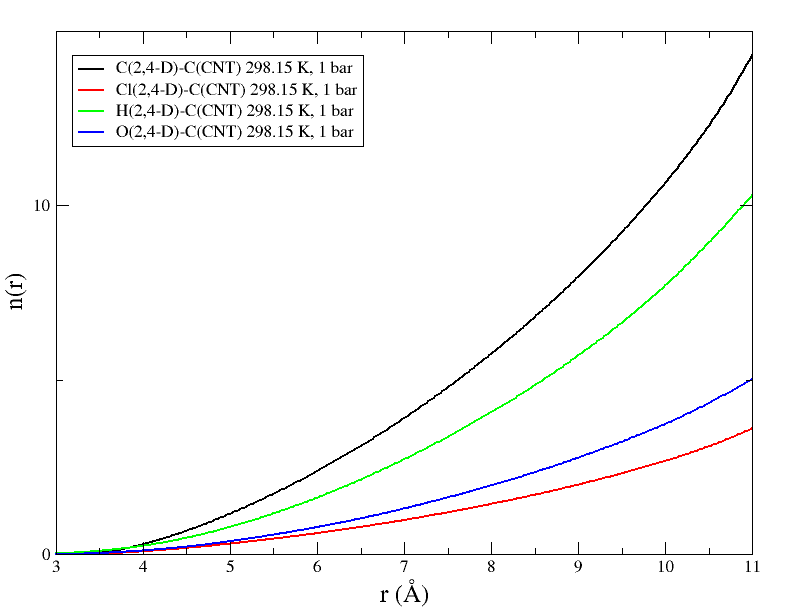
\includegraphics[width=1\linewidth]{resultados/gr_24D_CNT_298_15_atom_atom_cn_alt.png}  
  \caption{Número de coordinación de átomos C, Cl, H y O del herbicida con átomos C del nanotubo.}
  \label{fig:24D_CNT_298_15_atom_atom_cn}
\end{subfigure}
\begin{subfigure}{.5\textwidth}
  \centering
  % include second image
  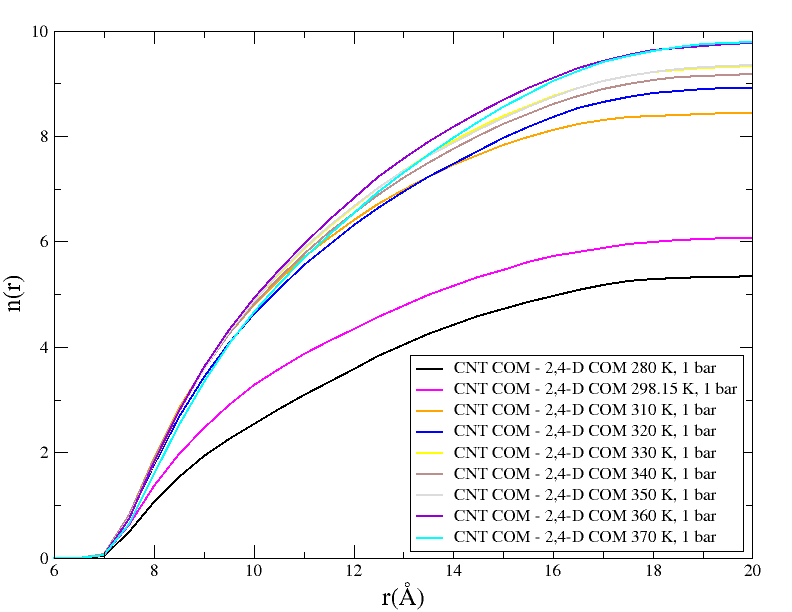
\includegraphics[width=1\linewidth]{resultados/cmnt_cmd_alltemp.png}  
  \caption{Número de coordinación entre el centro de masa del nanotubo y los centros de masa de moléculas de herbicida 2,4-D en el rango de temperaturas 280-370 K.}
  \label{fig:24D_CNT_alltemp_CM-CM_cn}
\end{subfigure}
\caption{Números de coordinación}
\label{fig:24D_CNT_298_15_alltemp_atom_atom_cn}
\end{figure}

La figura \ref{fig:24D_CNT_298_15_atom_atom_cn} es el número de coordinación obtenido a partir de las funciones de distribución radial presentadas en la figura \ref{fig:24D_CNT_298_15_atom_atom} a 298 K  y 1 bar, se observa que a la distancia de 5 \AA\ hay aproximadamente un átomo de hidrógeno y de carbono en promedio. En la figura \ref{fig:24D_CNT_alltemp_CM-CM_cn} se presenta el número de coordinación entre el centro de masa del nanotubo y los centros de masa de moléculas de herbicida 2,4-D para temperatura de 280 a 370 K. En este caso hay dos observaciones importantes: la primera es que el número de moléculas alrededor del centro de masa del nanotubo aumenta con la temperatura y la segunda: a 12 \AA\  del centro de masa del nanotubo se encuentran entre 3 a 7 moléculas 2,4-D según la temperatura a la que se encuentra el sistema. En las figuras \ref{fig:24DCOM} y \ref{fig:CNTCOM} se observan los centros de masa de la molécula 2,4-D y del nanotubo de carbono respectivamente.\\

\begin{figure}[!h]
    \centering
    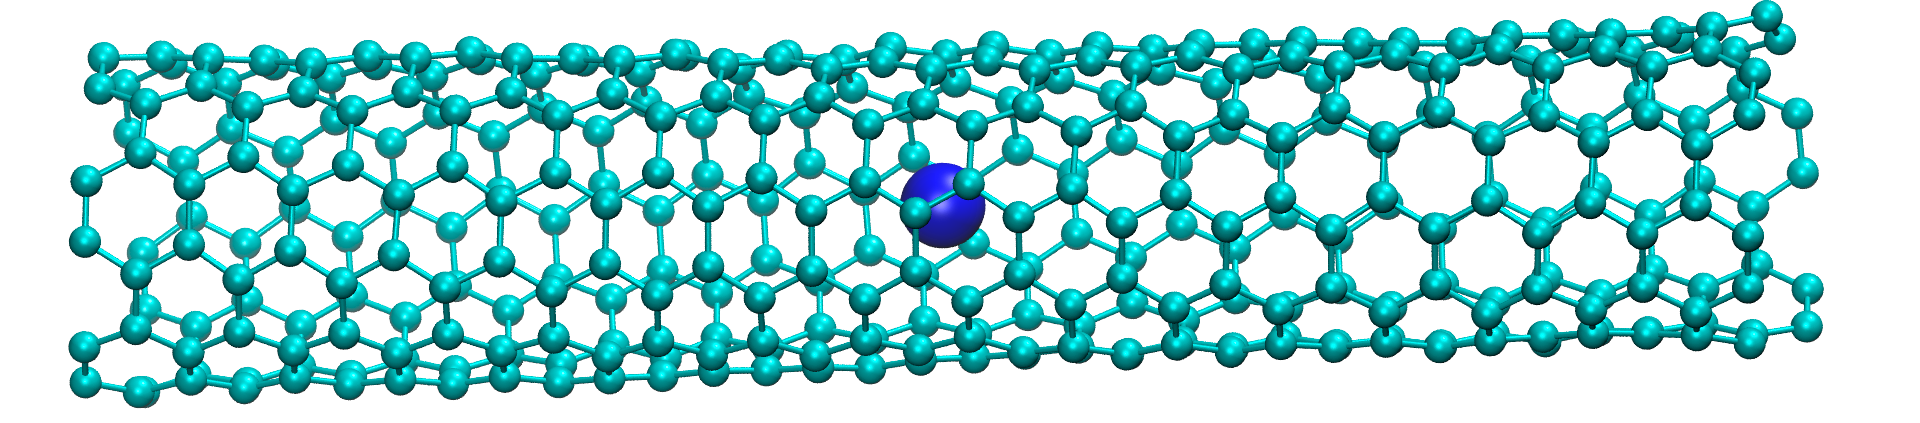
\includegraphics[width=.9\textwidth,keepaspectratio=true]{resultados/CNTCOM.png}
    \caption{Centro de masa del nanotubo de carbono (6,5), estudiado en esta tesis y representado por la esfera azul.}
    \label{fig:CNTCOM}
\end{figure}

\begin{figure}[!h]
    \centering
    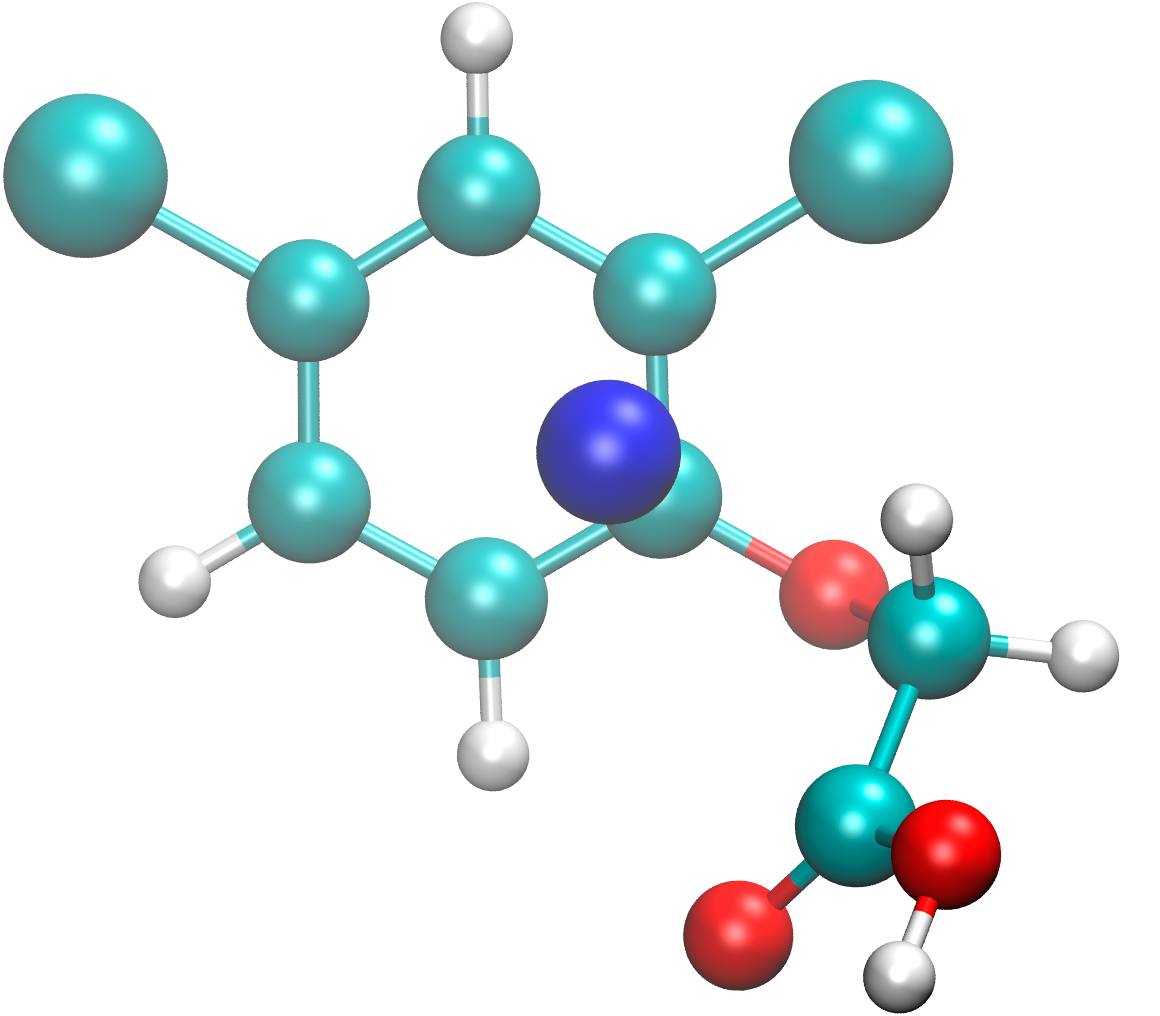
\includegraphics[width=.3\textwidth,keepaspectratio=true]{resultados/24DCOM.png}
    \caption{Centro de masa de la molécula de 2,4-D representado por la esfera azul.}
    \label{fig:24DCOM}
\end{figure}

\newpage

Todas las funciones de correlación indican una cercanía y una interacción atractiva que favorece un efecto adsorbente de la molécula de herbicida con la superficie del nanotubo de carbono. Esto se observa visualmente para todas las temperaturas estudiadas, por ejemplo, en la figura \ref{fig:Conffinal370}. 

\section{Desplazamiento cuadrático medio y coeficiente de difusión}

La figura \ref{fig:msd_all_298} es el desplazamiento cuadrático medio de las diferentes especies moleculares en el sistema a 298.15 K y 1 bar por 20000 ps de tiempo.

\begin{figure}[!h]
    \centering
    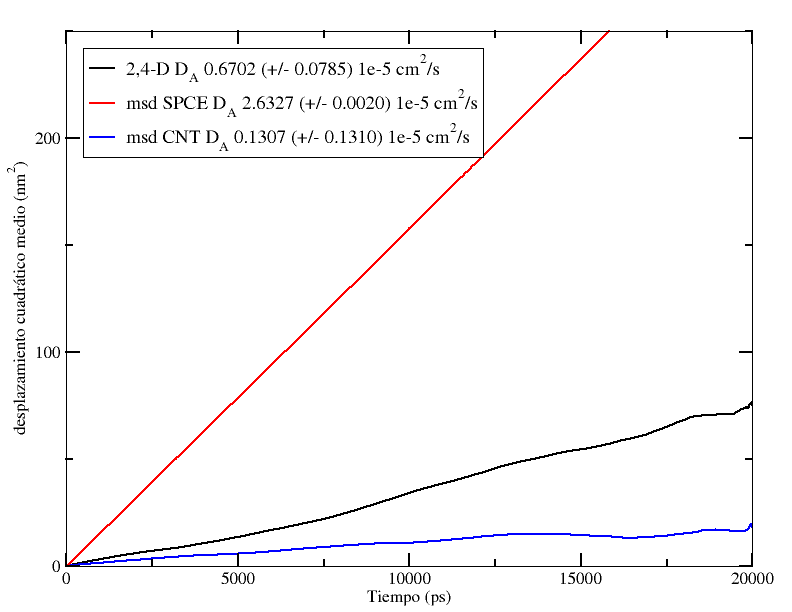
\includegraphics[width=.8\textwidth,keepaspectratio=true]{resultados/msd_all_29815.png}
    \caption{Desplazamiento cuadrático medio de herbicida 2,4-D, agua y nanotubo de carbono a 298.15 K.}
    \label{fig:msd_all_298}
\end{figure}

En la figura \ref{fig:comparación_msd_cnt_24d_340-370}, se presenta que el desplazamiento cuadrático medio del nanotubo de carbono y las moléculas 2,4-D a diferentes temperaturas y presión de 1 bar. Las curvas roja y negra son el desplazamiento del nanotubo y del herbicida a 370 K, respectivamente, observamos que son similares en forma lo que sugiere una alta correlación entre ambas especies moleculares y refuerza la observación de que hay una atracción dominante entre ellas, dando lugar al complejo que se observa, en la figura \ref{fig:Conffinal370}. \\

Un comportamiento similar se observa de 350 y 360 K. Sin embargo, para la temperatura de 340 K las curvas de desplazamiento cuadrático medio de nanotubo y herbicida son considerablemente diferentes, para prácticamente todos los tiempos. Este hallazgo sugiere que a estas condiciones el herbicida se mueve mas libremente respecto al nanotubo y la atracción entre estas especies es menor.\\

\begin{figure}[!h]
    \centering
    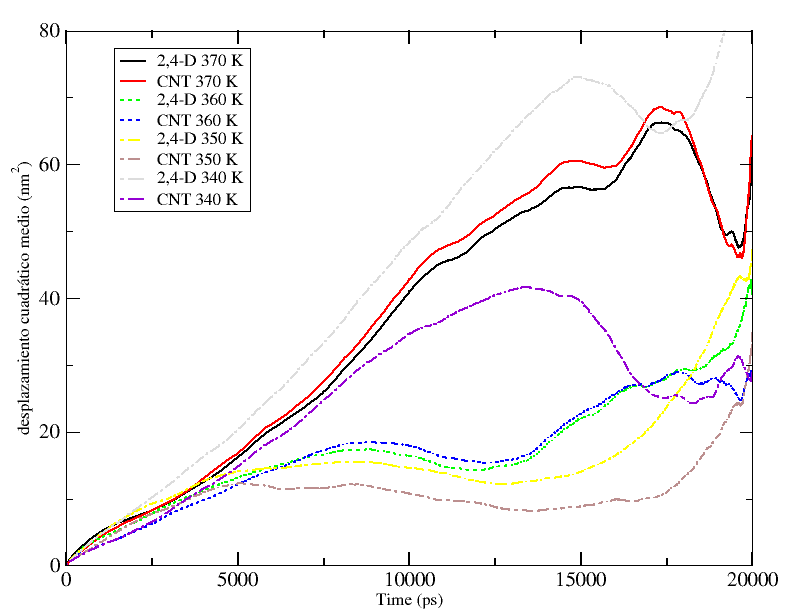
\includegraphics[width=.8\textwidth,keepaspectratio=true]{resultados/comparacion_msd_cnt_24d_340-370.png}
    \caption{Desplazamiento cuadrático medio del nanotubo de carbono y de las moléculas 2,4-D en el rango de temperaturas 340-370 K a 1 bar.}
    \label{fig:comparación_msd_cnt_24d_340-370}
\end{figure}

En la tabla \ref{tab:coefdifall} se presentan los coeficientes de difusión de las 3 especies moleculares del sistema y en el rango de temperaturas estudiado en esta tesis.\\

\newpage

\begin{table}[h!]
    \centering
    \begin{tabular}{ |m{8em}|m{3em}|m{3em}|m{5em}|m{3em}|m{3em}|m{3em}|  }
    \hline
    \multicolumn{7}{|c|}{Coeficiente de difusión $D_A$ $10^{-9}m^2/s$} \\
    \hline
    Temperatura (K) & 2,4-D & error & CNT (6,5) & error & SPCE & error\\
    \hline
    280 &  0.2549 & 0.0975 & 0.1105 & 0.0404 & 1.7348 & 0.0012\\
    \hline
    298.15 &  0.6702 & 0.0785 & 0.1307 & 0.1310 & 2.6327 & 0.0020\\
    \hline
    310 &  0.2625 & 0.0838 & 0.0321 & 0.2545 & 3.3389 & 0.0013\\
    \hline
    320 &  0.2031 & 0.0464 & 0.0705 & 0.0035 & 3.9671 & 0.0150\\
    \hline
    330 &  0.2521 & 0.1335 & 0.1934 & 0.1735 & 4.6600 & 0.0308\\
    \hline
    340 &  0.7448 & 0.4453 & 0.3052 & 0.8964 & 5.4419 & 0.0279\\
    \hline
    350 &  0.0701 & 0.0707 & 0.01204 & 0.04918 & 6.1984 & 0.0287\\
    \hline
    360 &  0.1672 & 0.1253 & 0.1890 & 0.0186 & 7.1217 & 0.0473\\
    \hline
    370 &  0.6641 & 0.1943 & 0.6959 & 0.2330 & 7.9940 & 0.0544\\
    \hline
    \end{tabular}
    \caption{Coeficientes de difusión de las 3 especies moleculares en el rango de 280 a 370 K a 1 bar.}
    \label{tab:coefdifall}
\end{table} 

Al analizar los datos de difusión observamos que a medida que la temperatura aumenta, el coeficiente de difusión del herbicida fluctúa entre 0.07 y 0.74 $10^{-9}m^2/s$. Para el nanotubo de carbono los valores del coeficiente son menores  pero el comportamiento es muy parecido al del herbicida, apoyando la idea  de que efectivamente esta especies se mueven acopladas entre si. En contraposición, el coeficiente del agua en la mezcla aumenta con la temperatura, de manera similar a como lo hace el agua pura \cite{moultos2018} indicando que el comportamiento del agua en la mezcla no es modifica considerablemente con respecto a su valor en agua pura.

\begin{figure}[!h]
    \centering
    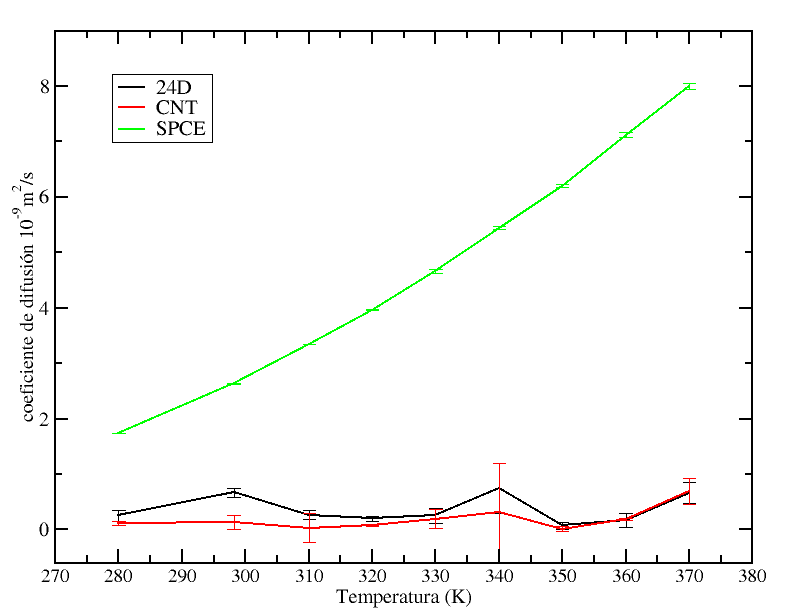
\includegraphics[width=.8\textwidth,keepaspectratio=true]{resultados/coefdif.png}
    \caption{Desplazamiento cuadrático medio de las moléculas contra la temperatura de 280 a 370 K a 1 bar.}
    \label{fig:coeficientemoleculas}
\end{figure}

% -------------------------------------------------------------------
% Funciones g(r)  [átomo A - átomo B]
% -------------------------------------------------------------------
% agua-agua:  g_OO,  g_OH,  g_HH   en funcion de la T (275 - 370 K) 
% agua-42D:   g_(OW-OD), g_(HW-HD), g_(OW-ClD), g_(HW-ClD), g_(OW-HD)
% agua-CNT:  g_(OW-C),  g_(HW-C)

% 42D-CNT:  g_(OD-C),  g_(HD-C),  g_(ClD-C),  g_(CD-C)
% 42D-42D:   g_(OD-OD),  g_(HD-HD),  g_(ClD-ClD),  g_(CD-CD),  g_(ClD-HD),  g_(OD-HD)

% CNT-CNT:   g_(C-C)
% ------------------------------------------------------------------------
% Funciones g(r)  [cm M - cm N]
% ------------------------------------------------------------------------
% CNT-42D:   g_(cm CNT - cm D),  g_(cm tapa CNT - cm D)

% ------------------------------------------------------------------------ 
% Funciones g(r)  [cm M -  átomo B]
% ------------------------------------------------------------------------
% CNT-42D:  g_(cm NT - ClD),  g_(cm NT - HD),  g_(cm NT - OD),  g_(cm NT - Cl1D), g_(cm NT - OD)
% CNT-agua:  g_(cm NT - OW),  g_(cm NT - HW)

